\section{Train Custom Data: Weights, Biases Logging, Local Logging}

\begin{figure}[h]
    \centering
    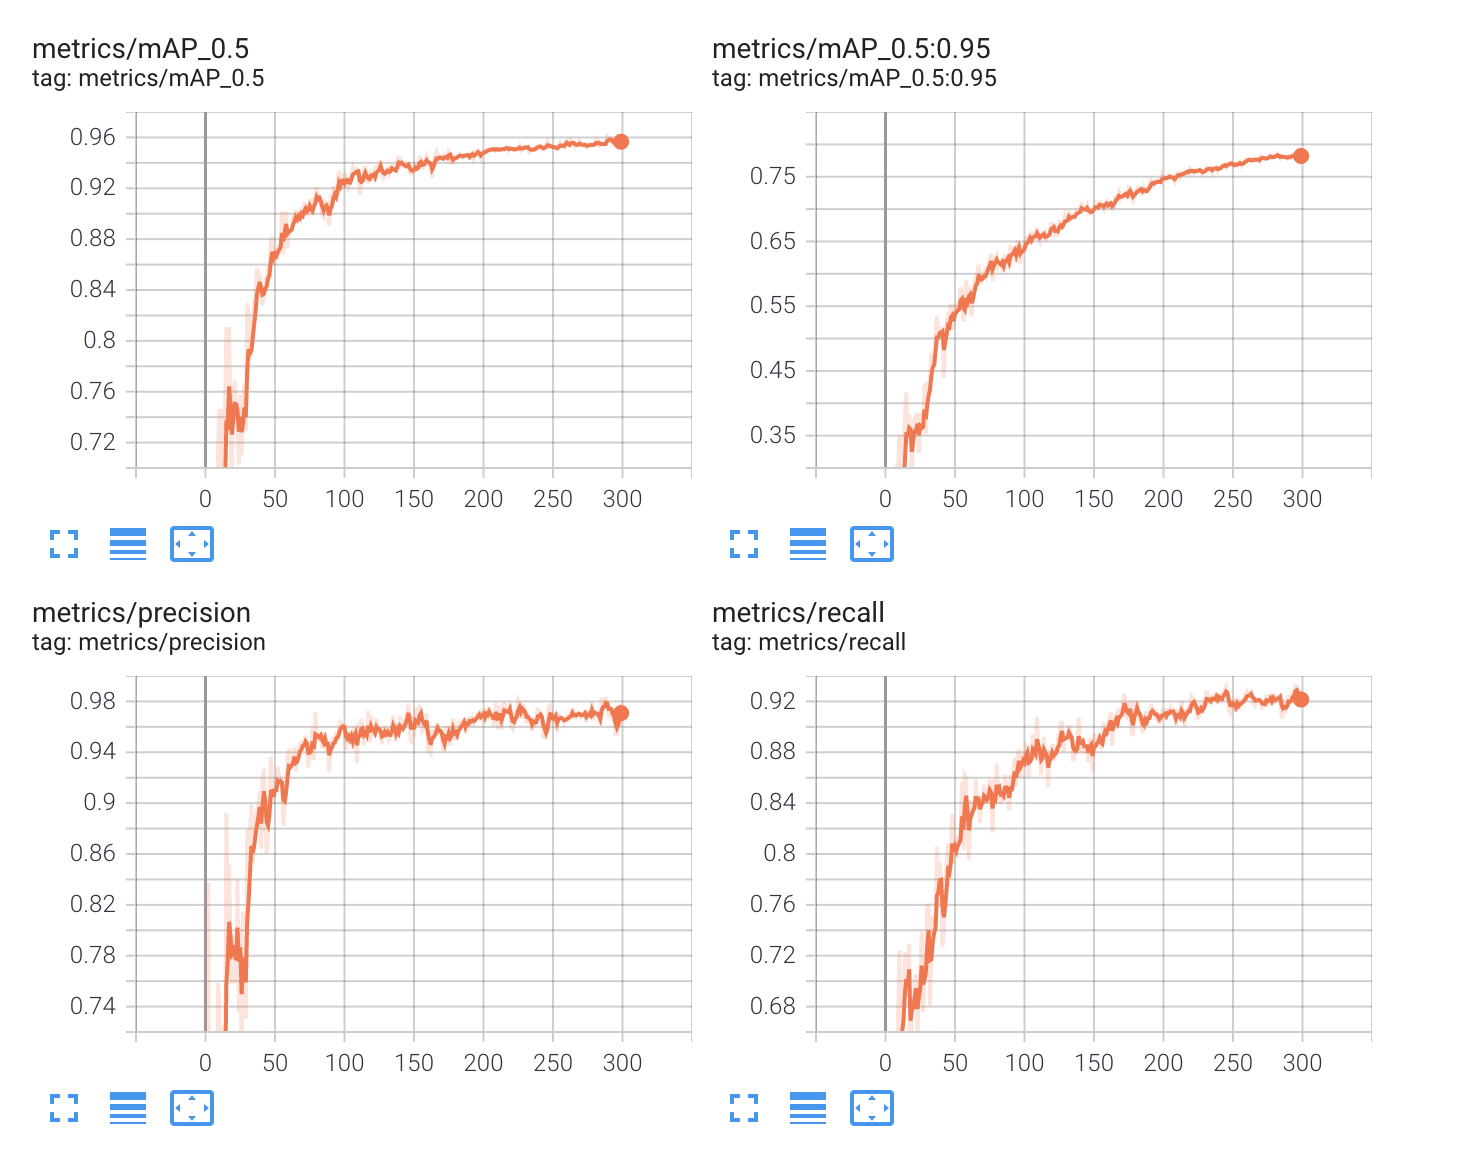
\includegraphics[scale=0.43]{img/colab_metrics.png}
    \caption{Average model precision when IOU is larger than 0.5; Average model precision when IOU is between 0.5 and 0.95; The model precision; The model recall rate.}
    \label{fig:colab_metrics}
\end{figure}


As described in Sec~\ref{sec:3.1}, 694 satellite images with a resolution of 4800x2908 were rescaled to a size of 416x416. This can greatly improve the efficiency of training the model. It is a fact that with the training of a model with 47 million parameters, the precision and recall of the training results improved significantly with the number of training sessions.

As shown in Figure~\ref{fig:colab_metrics} above, the average accuracy of the model, the precision of the model and the recall of the model all show a significant increase with the number of times the model is trained when the IOU\footnote{Intersection over Union is an evaluation metric used to measure the accuracy of an object detector on a particular dataset.} (Intersection over Union) is between 0.5 and 0.95. In particular, the precision of the model can eventually reach a level close to 98\%. However, this does not necessarily mean that the model will also fit satellite imagery of the Gulf of California. First, such high accuracy results only tell us that the model can achieve a relatively high recognition accuracy, which gradually increases and eventually reaches 98\% after 300 training repetitions. If the algorithm needs to be trained for this area, then consideration needs to be given to purposefully selecting many small boats in or near the area as a source of data for training the model. Secondly, there is also an inequity in the level of resolution of the training and test data.

To train the model faster, I reduced the resolution of the images by a factor of about 70 (from 4800x2908 pixels to 416x416 pixels). Otherwise, the training could take half a month if used images with a resolution of 4800x2908 pixels as the data source! However, each image from the Gulf of California was maintained at a resolution of 4K (3840x2160 pixels). This would result in the algorithm not framing the target perfectly when it detects it, i.e., it would not be perfectly tangential to the edges of the target.

Similarly, as shown in Figure~\ref{fig:colab_train} below, the loss rate of the box can eventually reach 1\% as the number of training sessions increases. Since this thesis has defined only one class of object, i.e. boat, this means that the probability that the detection box does not detect that it is a boat at all is 1\%. Similarly, because there is only one class, the class loss rate is 0. Figure~\ref{fig:test_batch1_pred} below shows the prediction results during the training of the model, it can be seen that the model is able to detect the occurrence of boats 100\% of the range tested and gives the corresponding range box. Most of the detected boats were mostly considered to have a 90\% probability of being boats. Since only one class was set, some were also considered to have a 100\% probability of being boats.



\begin{figure}[!h]
    \centering
    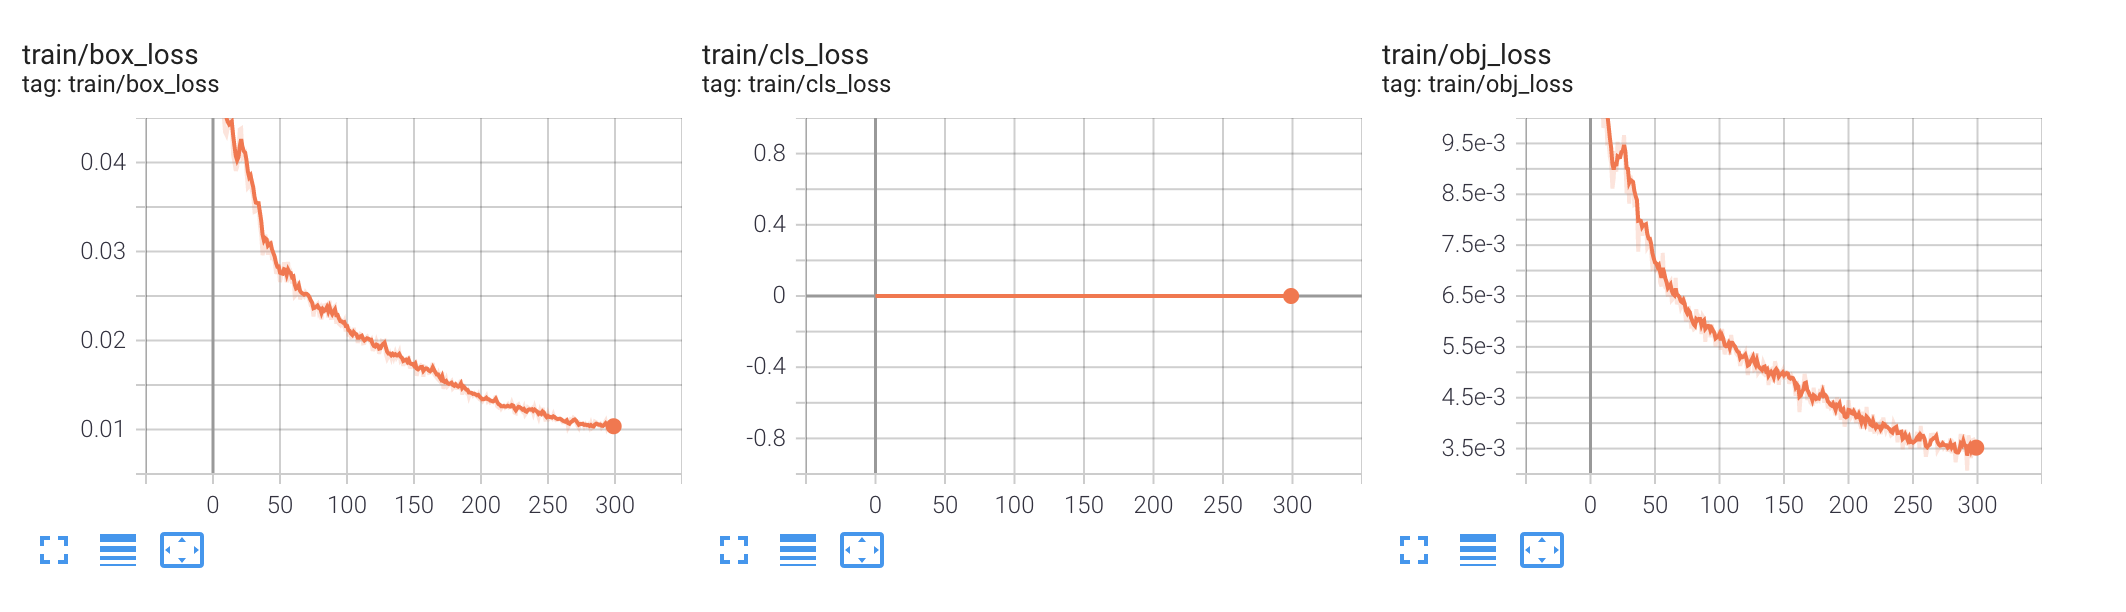
\includegraphics[scale=0.4]{img/colab_train.png}
    \caption{The box loss rate of the model; The class loss rate of the model; The object loss rate of the model.}
    \label{fig:colab_train}


    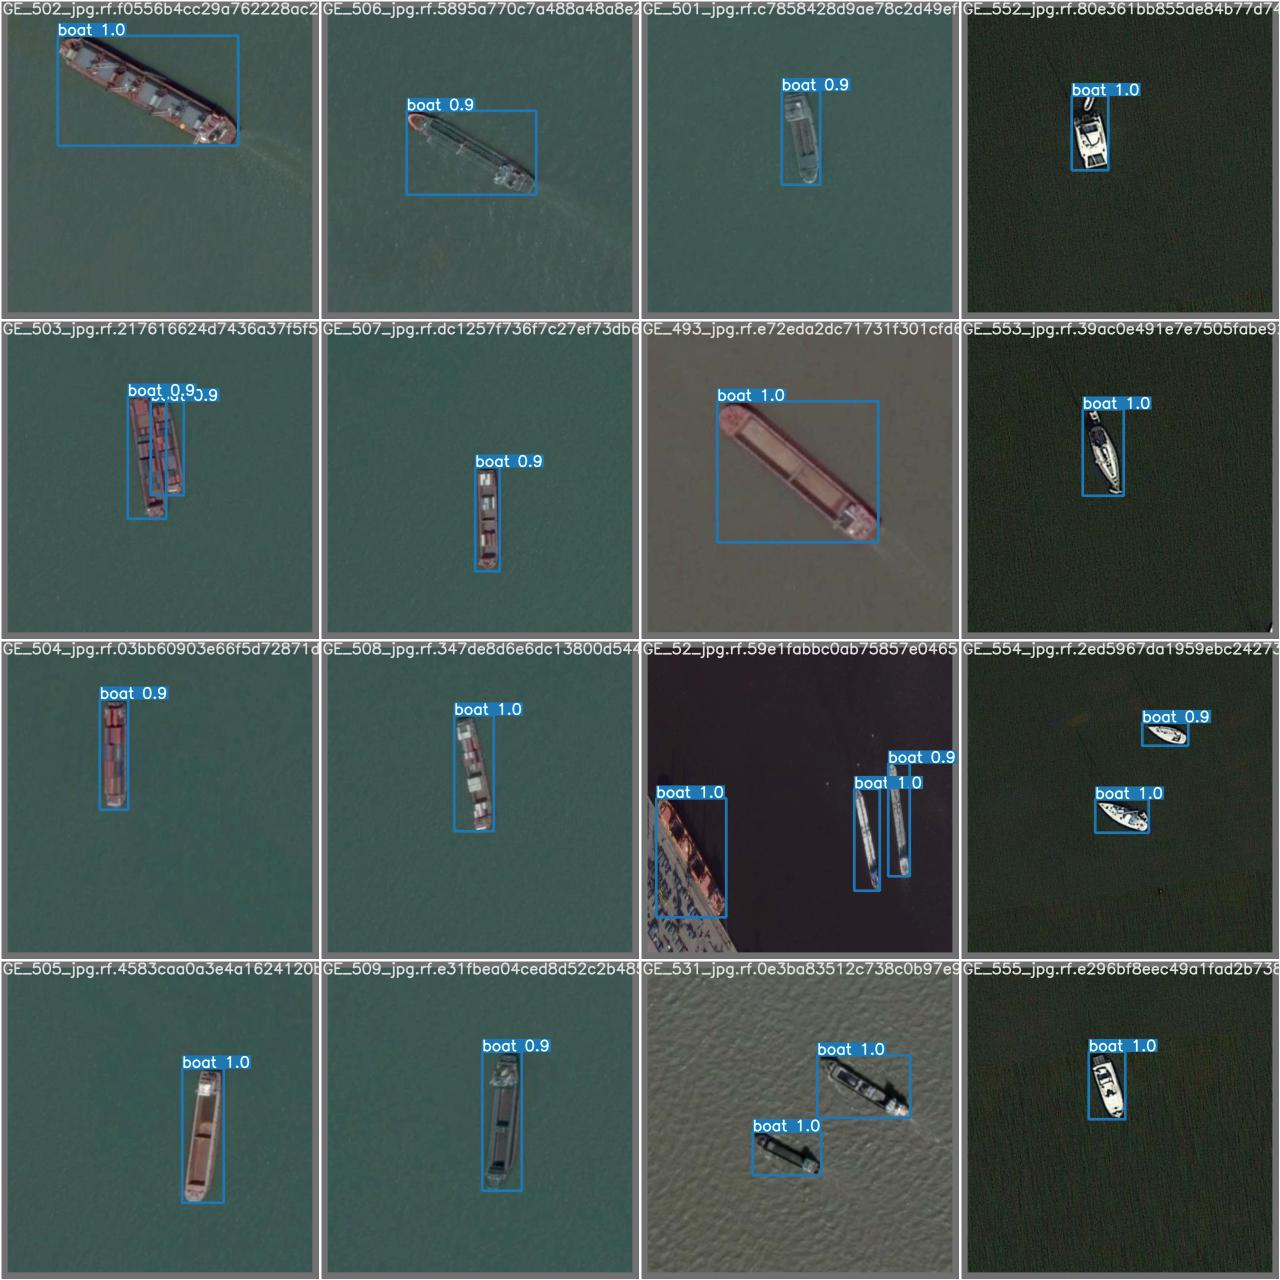
\includegraphics[scale=0.25]{img/test_batch1_pred.jpg}
    \caption{Test result of a trained model for detecting ships.}
    \label{fig:test_batch1_pred}
\end{figure}


\newpage
\section{Detection Results and Vessel Composition}

In Sec~\ref{sec3.2.3}, I discussed the method of detecting small boats. Most for the result, I will test the length of two small boats on a certain sea. The results are shown in Figure~\ref{fig:length_test}. A smaller boat shown in a Google Earth Pro image measured 6.98 meters, while the algorithm detected a length of 6.744 meters. The error between them is 3.38\%. The other larger boat Google Earth Pro measured 41.38 meters in length, and the algorithm detected 40.984 meters. The error between them is 0.96\%. After testing, the length of the boat detected by the algorithm was within an acceptable error range.

\begin{figure}[h!]
    \centering
    \includegraphics[scale=0.4]{img/length_test.png}
    \caption{Test the length of boat.}
    \label{fig:length_test}
\end{figure}



As explained in Sec~\ref{sec3.2.1}, it was unwise to select the entire region for the study due to the uneven amount of data that Google Earth Pro has provided for the Gulf of California over the past three years. Therefore, three areas with more data were chosen: Santa Rosalia, Loreto, and Guaymas. Ultimately, satellite images of these three areas were found for 2019, 2020, and 2021, for a total of 690 images. Each of the 690 images is a satellite image with an eye altitude of 200 metres and a resolution of 3840x2160 pixels.

However, as stated in Sec~\ref{sec3.2.2}, some of the slightly earlier satellite images had inferior detail representation capabilities, which resulted in the model not being very good at accurately detecting the features of the target, so that many small boats in the Gulf of California could not actually be detected. However, after enhancement with the 5x5 sharpening kernel, the recognition rate of the model was significantly improved. However, the following situations still occur.

\begin{enumerate}[(a)]
    \item  Figure~\ref{fig:1_docked_together_Guaymas_202001_20}: When the detailed representation of the image is indigent and two or three small boats are moored together, the model is very likely to recognise the two or three boats as a whole. There are two reasons for this problem. One is that the training data is mostly a `fuzzy' data source. Thus, when there are two or three small boats moored together, the model cannot easily detect the features of each small boat individually. In contrast, it may seem more reasonable to the model that the two or three boats as a whole have the same features. The second reason is that most data sources are individual boats on the surface or boats docked close to each other. As the data sources do not fully consider the fuzzy nature of the detail needed to detect the data and the fact that they are too close together, the model naturally does not recognise such cases.
    
    \item Figure~\ref{fig:2_square_Guaymas_202001_01}: When a cargo ship is moored on the shore, the ship and cargo appear as a 'rectangle' from the sky, much like a long jetty, and therefore sometimes cannot be detected. This is because small ships with a rectangular shape are not common in the preparation of data sources. This also applies to uncommon vessels such as battleships. 

    \item Figure~\ref{fig:3_beach_SantaRosalia_202104_02}: The recognition rate is also significantly lower when the boat is sometimes parked on the beach rather than on the water. This is also because most of the data was based on data on the water rather than on boats on the beach when the model was trained.

\end{enumerate}

\begin{figure}[p]
    \centering
    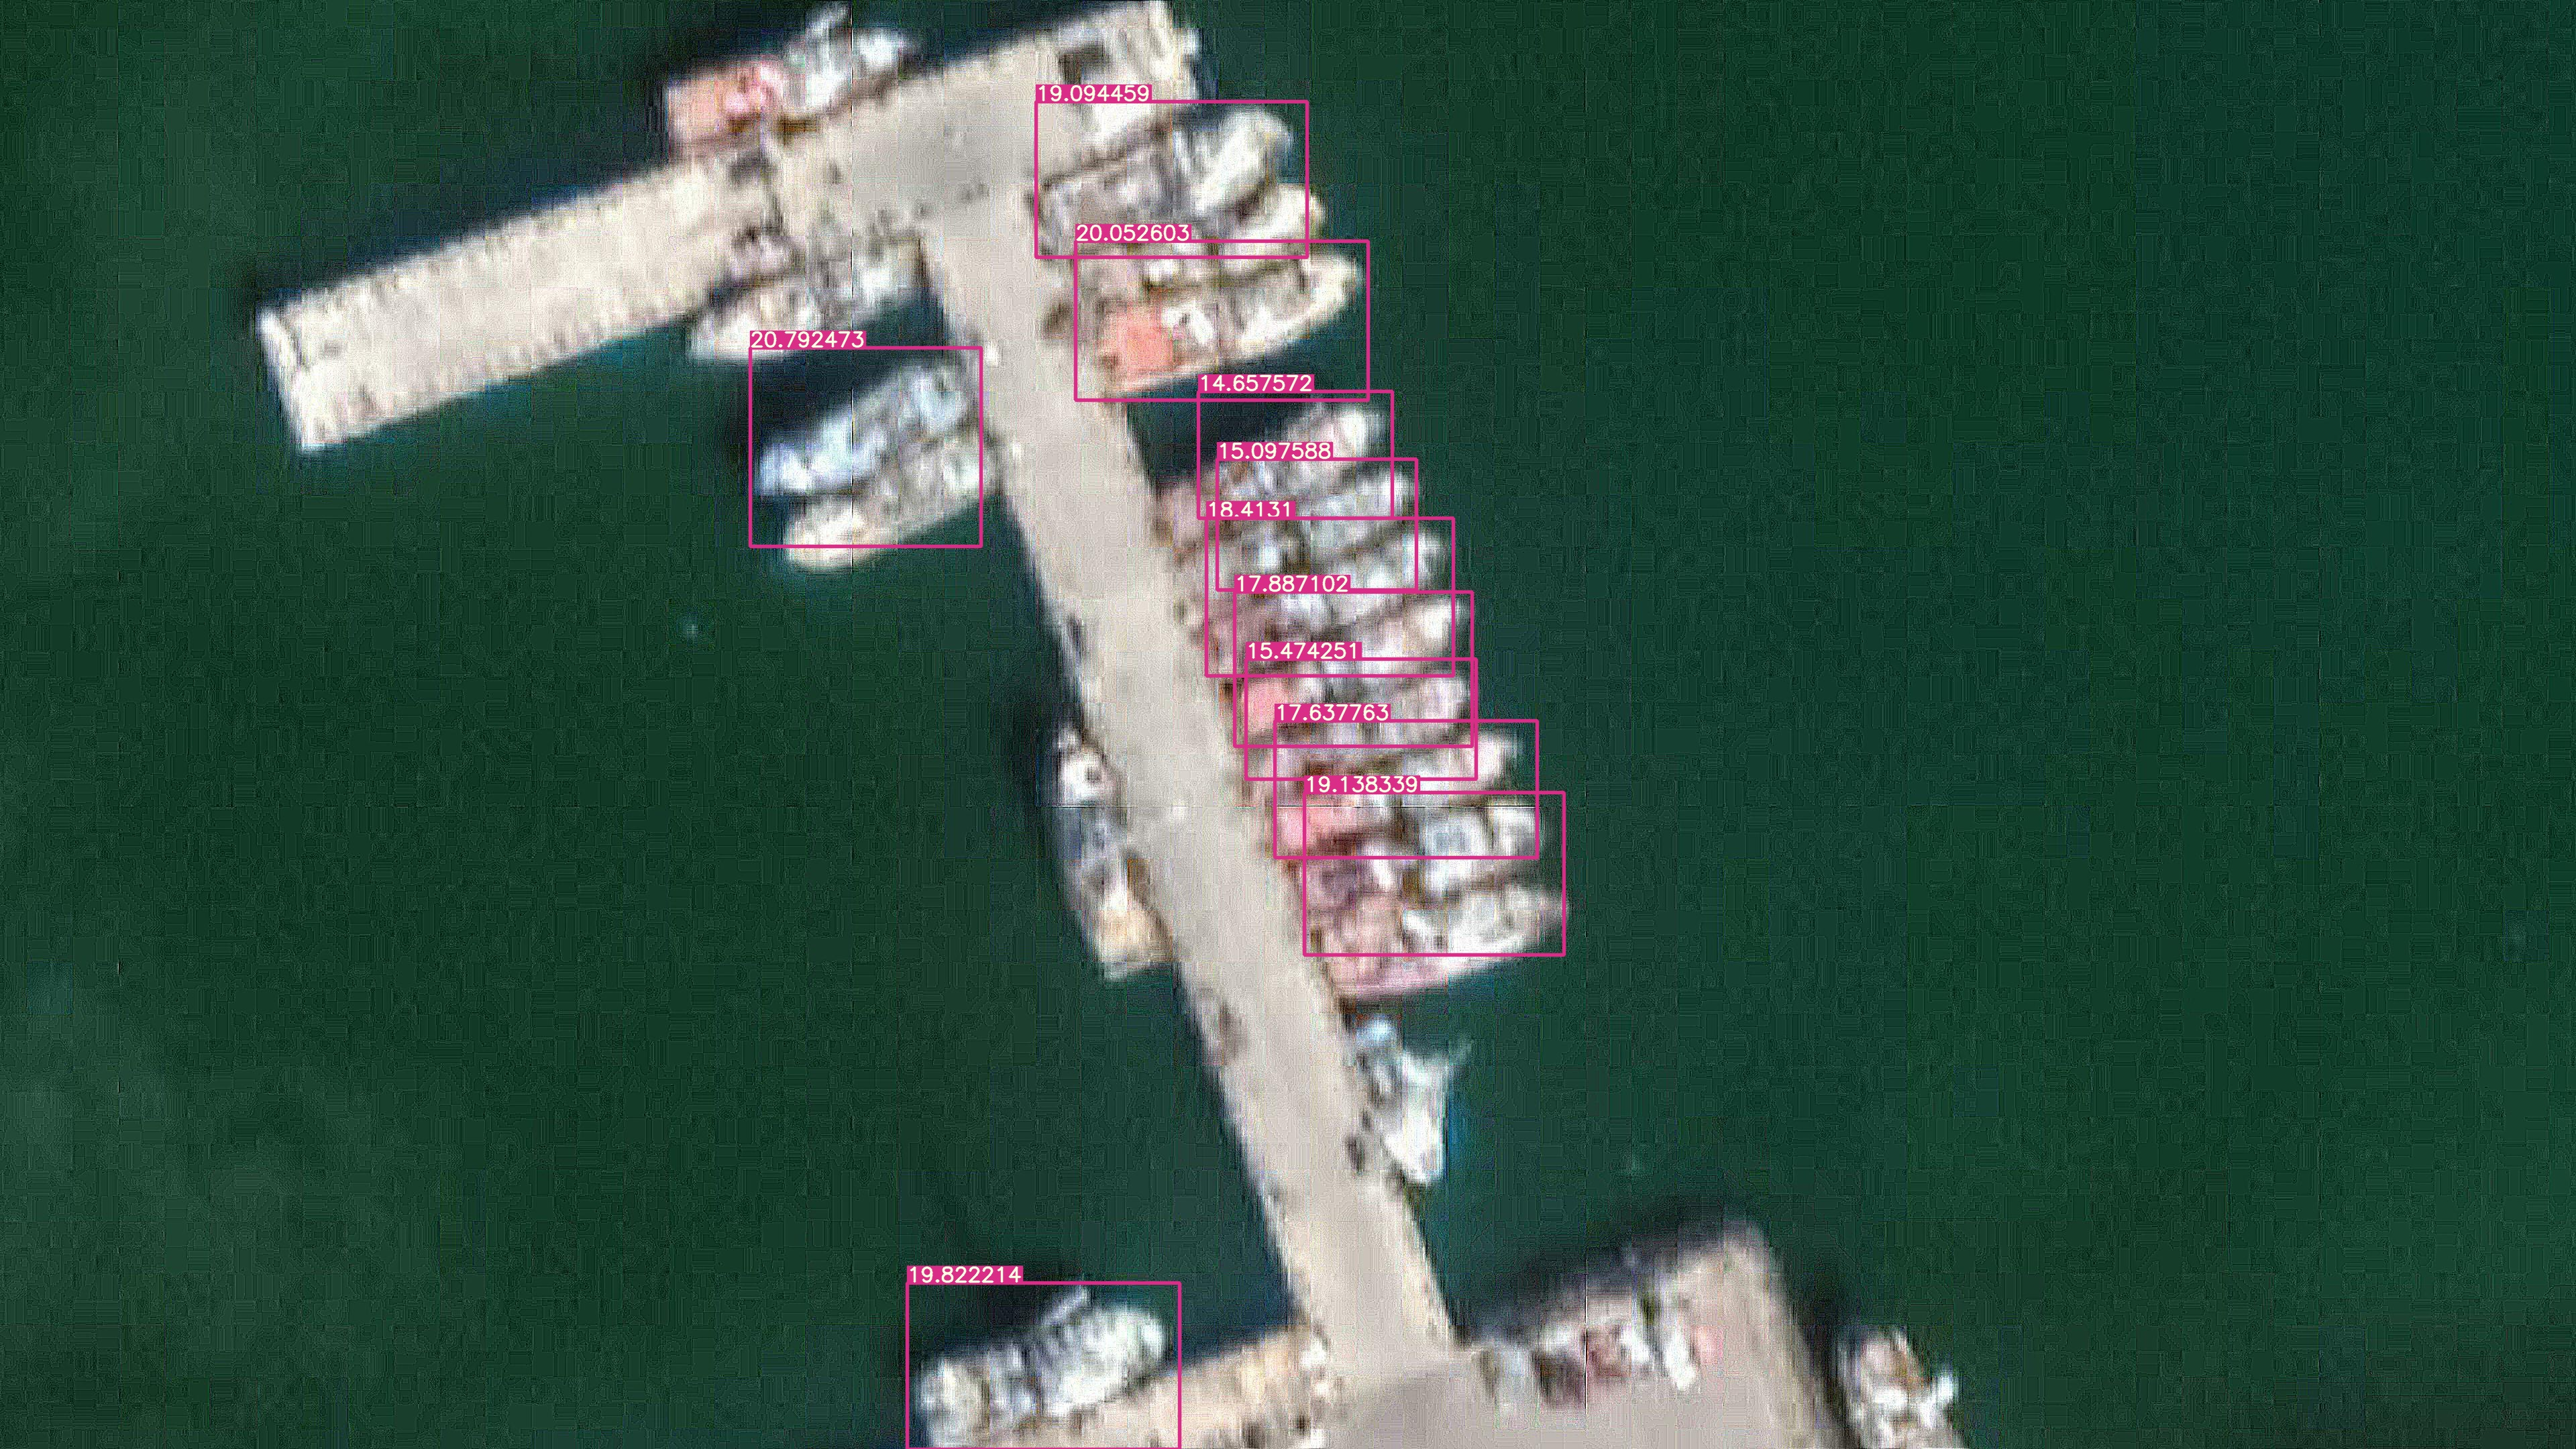
\includegraphics[scale=0.08]{img/1_docked_together_Guaymas_202001_20.jpg}
    \caption{When small boats are moored closely together in the harbour, the model may recognise two small boats as one. Image is from Guaymas, Jan 2020.}
    \label{fig:1_docked_together_Guaymas_202001_20}


    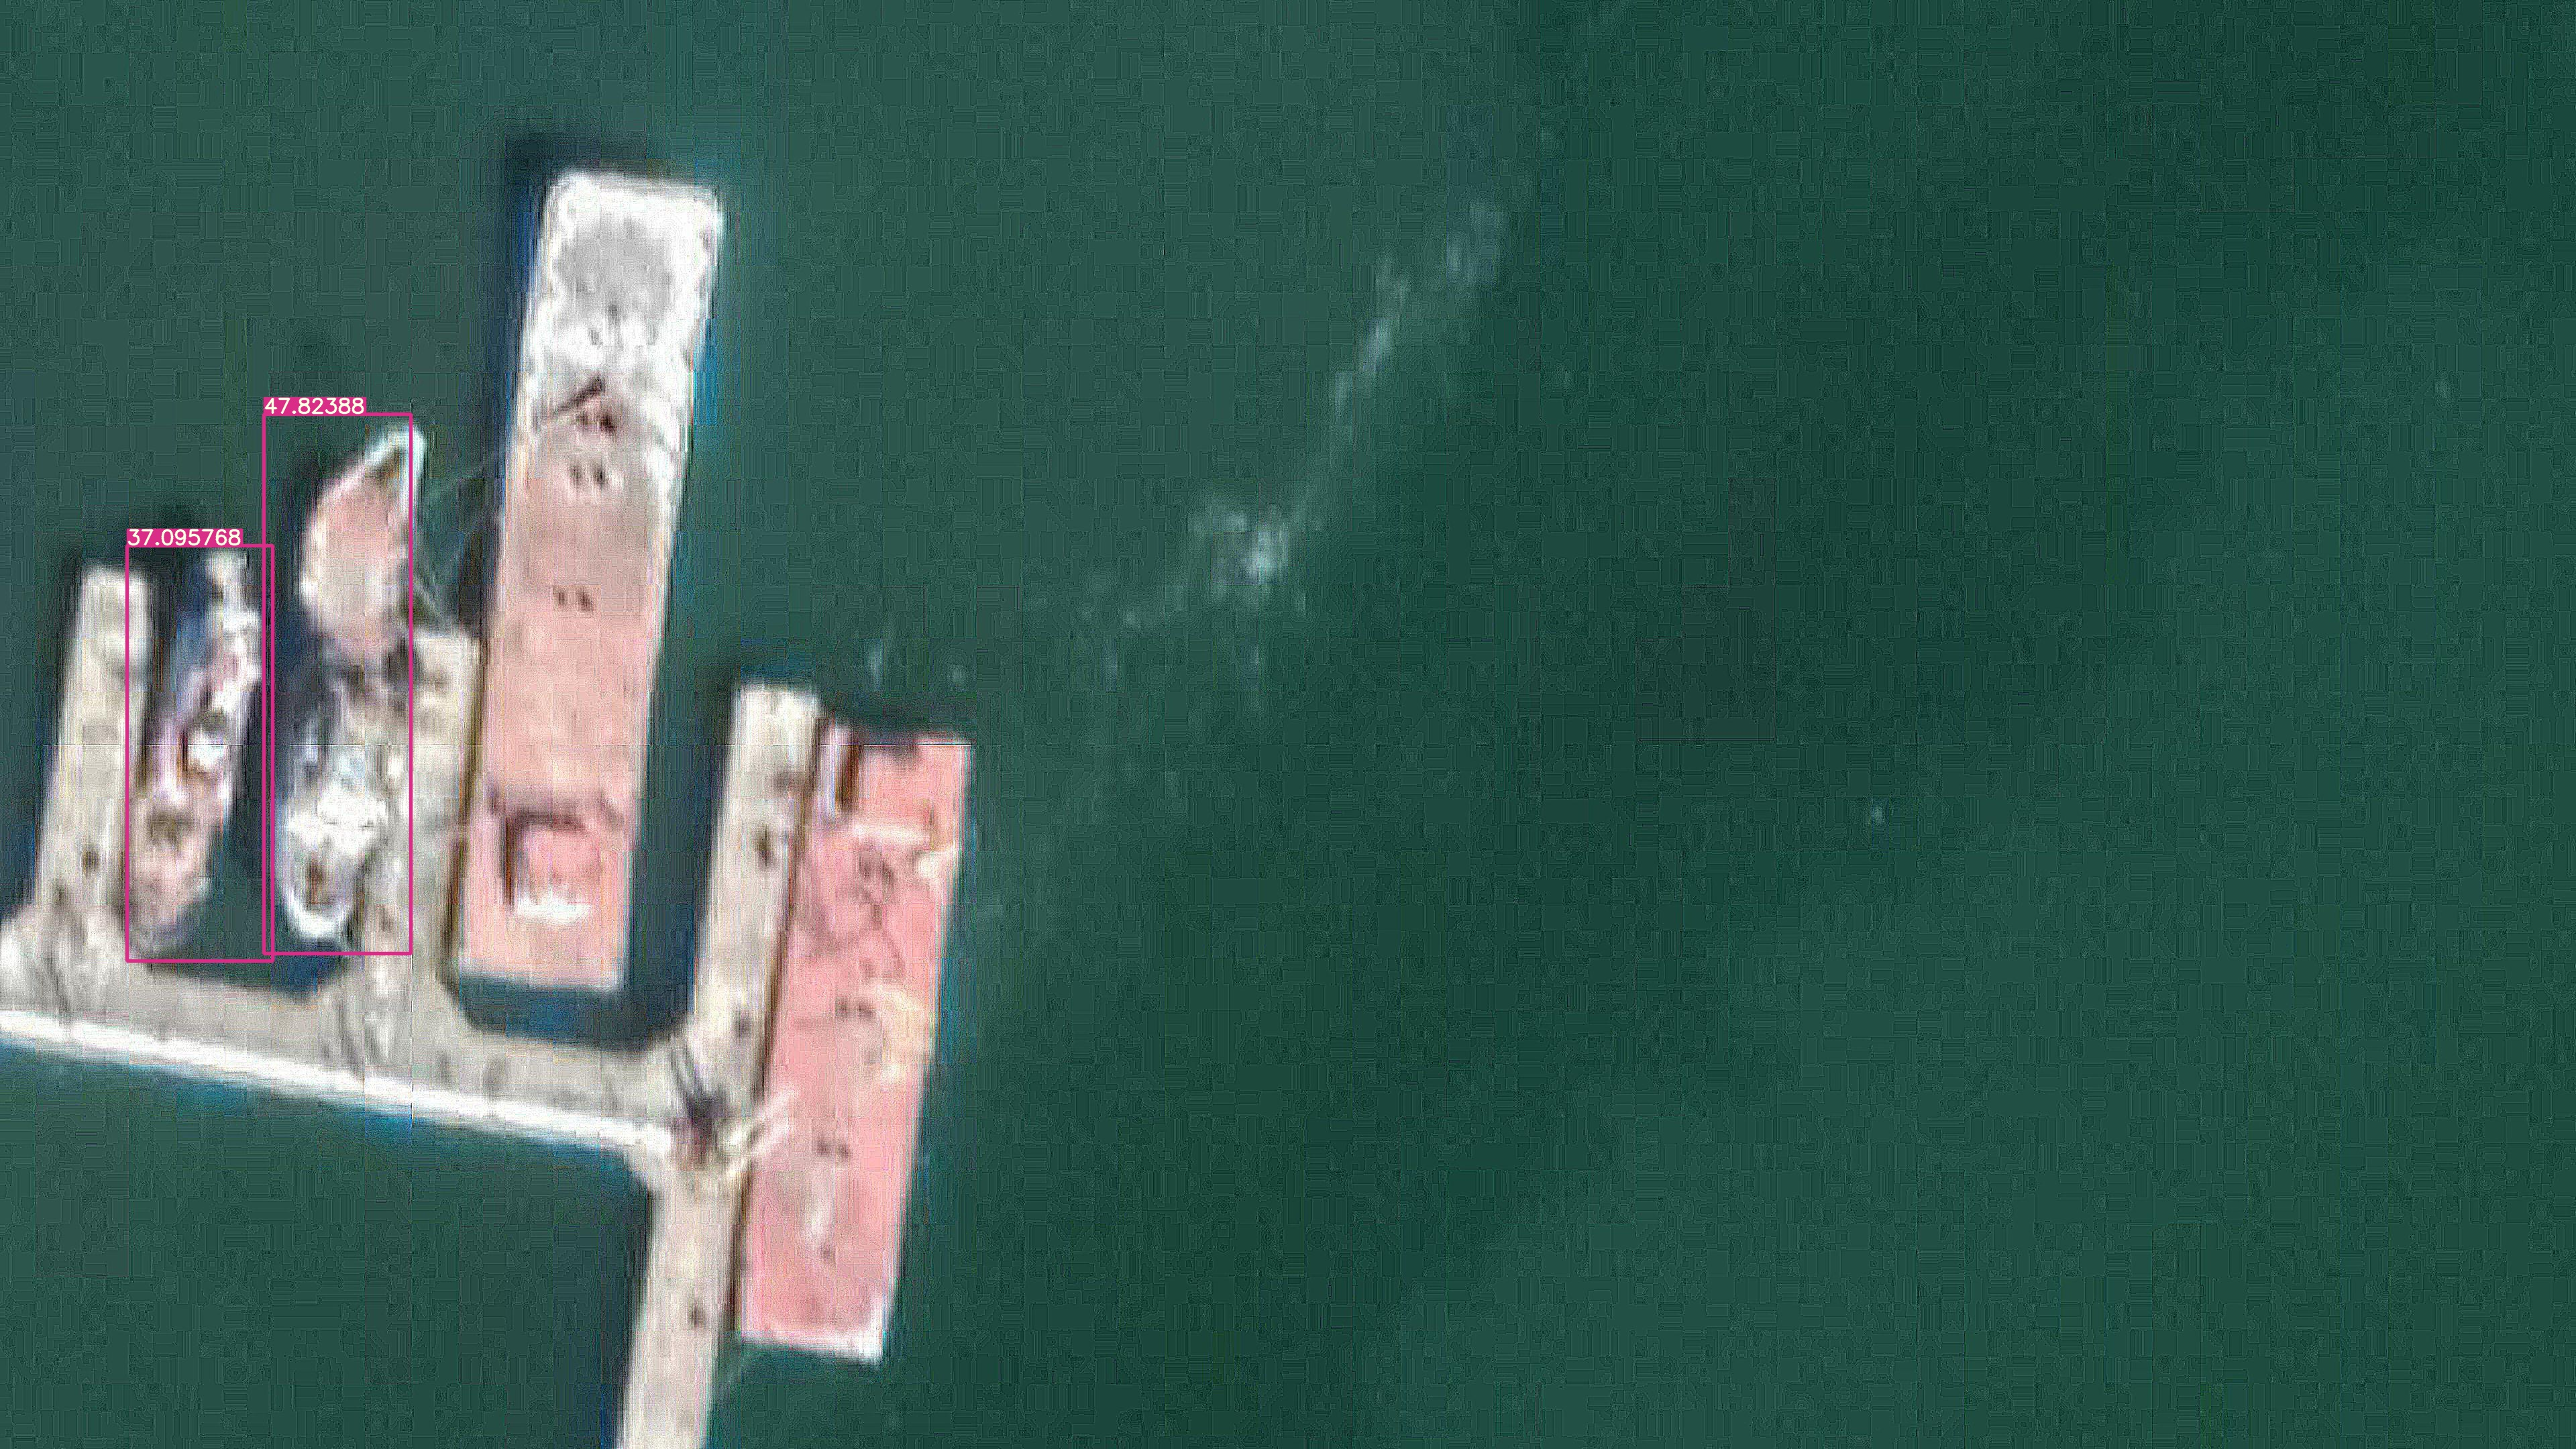
\includegraphics[scale=0.08]{img/2_square_Guaymas_202001_01.jpg}
    \caption{When the cargo ship is full of cargo, the ship looks like a rectangular jetty from above and loses the normal shape of a ship. Image is from Guaymas, Jan 2020.}
    \label{fig:2_square_Guaymas_202001_01}


    \includegraphics[scale=0.08]{img/3_beach_SantaRosalia_202104_02.jpg}
    \caption{Models may have difficulty detecting small boats moored on the beach. Image is from SantaRosalia, Feb 2021.}
    \label{fig:3_beach_SantaRosalia_202104_02}
\end{figure}

\newpage
Nevertheless, as Figure~\ref{fig:1_docked_together_Guaymas_202001_20}, Figure~\ref{fig:2_square_Guaymas_202001_01}, Figure~\ref{fig:3_beach_SantaRosalia_202104_02} demonstrate, the model still detects most of the small boats in the poorly detailed satellite images. A Python script was then designed to count the number of small and large boats between regions. The results (Table~\ref{table:4.1} to Table~\ref{table:4.9}) are shown below.


\begin{table}[h!]
\begin{tabular}{|l|l|l|l|l|l|l|l|l|}
\hline
                                       & Jan & Feb & Mar & Apr & Jun & July & Sep & Nov \\ \hline
Boats length \textless 24 meters       & 115 & 83  & 99  & 131 & 82  & 107  & 90  & 98  \\ \hline
Boats length \textgreater{}= 24 meters & 31  & 24  & 21  & 24  & 22  & 22   & 21  & 19  \\ \hline
\end{tabular}
\caption{Small ships and large ships in Guaymas in 2019.}
\label{table:4.1}



\begin{tabular}{|p{2.4cm}|l|l|l|l|l|l|l|l|l|l|l|}
\hline
                                       & Jan & Feb & Mar & Apr & May & Jun & July & Aug & Sep & Nov & Dec \\ \hline
Boats length \textless 24 meters       & 63  & 101 & 159 & 52  & 145 & 85  & 66   & 121 & 28  & 74  & 113 \\ \hline
Boats length \textgreater{}= 24 meters & 18  & 13  & 15  & 13  & 21  & 4   & 13   & 22  & 15  & 28  & 15  \\ \hline
\end{tabular}
\caption{Small ships and large ships in Guaymas in 2020.}



\begin{tabular}{|l|l|l|l|l|}
\hline
                                       & Feb & Mar & Apr & May \\ \hline
Boats length \textless 24 meters       & 161 & 167 & 144 & 119 \\ \hline
Boats length \textgreater{}= 24 meters & 19  & 33  & 21  & 22  \\ \hline
\end{tabular}
\caption{Small ships and large ships in Guaymas in 2021.}
\end{table}


\begin{table}[h!]
\begin{tabular}{|l|l|l|l|l|l|l|l|l|}
\hline
                                       & Jan & Apr & Jun & July & Aug & Sep & Nov & Dec \\ \hline
Boats length \textless 24 meters       & 40  & 60  & 18  & 49   & 33  & 42  & 38  & 17  \\ \hline
Boats length \textgreater{}= 24 meters & 0   & 1   & 0   & 0    & 1   & 0   & 1   & 0   \\ \hline
\end{tabular}
\caption{Small ships and large ships in Loreto in 2019.}



\begin{tabular}{|l|l|l|l|l|l|l|l|l|l|}
\hline
                                       & Jan & Feb & Mar & Apr & Jun & July & Aug & Sep & Nov \\ \hline
Boats length \textless 24 meters       & 18  & 26  & 18  & 30  & 32  & 33   & 20  & 43  & 43  \\ \hline
Boats length \textgreater{}= 24 meters & 0   & 0   & 0   & 0   & 0   & 0    & 0   & 1   & 1   \\ \hline
\end{tabular}
\caption{Small ships and large ships in Loreto in 2020.}


\begin{tabular}{|l|l|l|l|}
\hline
                                       & Jan & Feb & Apr \\ \hline
Boats length \textless 24 meters       & 16  & 33  & 33  \\ \hline
Boats length \textgreater{}= 24 meters & 0   & 0   & 0   \\ \hline
\end{tabular}
\caption{Small ships and large ships in Loreto in 2021.}
\end{table}


\begin{table}[h!]
\begin{tabular}{|l|l|l|l|l|l|}
\hline
                                       & Jan & July & Aug & Sep & Dec \\ \hline
Boats length \textless 24 meters       & 27  & 41   & 36  & 29  & 22  \\ \hline
Boats length \textgreater{}= 24 meters & 0   & 2    & 1   & 0   & 2   \\ \hline
\end{tabular}
\caption{Small ships and large ships in Santa Rosalia in 2019.}

\begin{tabular}{|p{2.4cm}|l|l|l|l|l|l|l|l|l|l|l|}
\hline
                                       & Jan & Feb & Mar & Apr & May & Jun & July & Aug & Sep & Nov & Dec \\ \hline
Boats length \textless 24 meters       & 50  & 43  & 37  & 48  & 8   & 44  & 66   & 58  & 58  & 43  & 57  \\ \hline
Boats length \textgreater{}= 24 meters & 1   & 1   & 1   & 1   & 0   & 1   & 3    & 1   & 1   & 1   & 1   \\ \hline
\end{tabular}
\caption{Small ships and large ships in Santa Rosalia in 2020.}

\begin{tabular}{|l|l|l|}
\hline
                                       & Apr & May \\ \hline
Boats length \textless 24 meters       & 32  & 46  \\ \hline
Boats length \textgreater{}= 24 meters & 1   & 2   \\ \hline
\end{tabular}
\caption{Small ships and large ships in Santa Rosalia in 2021.}
\label{table:4.9}
\end{table}



\newpage
As can be seen from the nine tables above, Guaymas, Loreto and Santa Rosalia can be classed by two different types of port cities:

\begin{enumerate}
    \item Loreto and Santa Rosalia have a much smaller number of ships and almost no large ships larger than 24 metres in length.
    \item The port of Guaymas was probably much larger than that of Loreto and Santa Rosalia. There are about four times more small ships in Guaymas than in Loreto and about three times more small ships than in Santa Rosalia. The port of Guaymas has around 20 large ships per day, while Loreto has almost no large ships, and Santa Rosalia probably has at least one large ship per day.
\end{enumerate}

In addition to the number of ships in each port, another interesting finding is that the number of ships in Guaymas's port, in similar seasons, increases compared to the numbers in the previous year. In February, for example, the number of ships in 2019 is less than the number of ships in 2020, and the number of ships in 2020 is less than the number of ships in 2021. The reason for this could be the rapid development of the maritime industry in Guaymas in just three years. However, another potential reason is that the quality of satellite imagery in Guaymas in 2021 is much better than in 2020, resulting in almost 50\% more vessels being detected by the model in 2021 than in 2020.

Similarly, the quality of satellite imagery in the Guaymas area in 2020 is also better than in 2020, resulting in almost 25\% more ships being detected by the model in 2020 than in 2019. The same thing happened in Santa Rosalia. For instance, in July, there were nearly 50\% more small ships in Santa Rosalia in 2020 than in 2019.

However, this does not always happen. In fact, as the satellite images of Loreto have not improved significantly in the last three years, such a conclusion does not hold. Besides, it is also difficult to encapsulate the 2021 data in this conclusion due to the large blank in the 2021 Santa Rosalia data.



\section{Entertainment Boats in the Gulf of California}
According to the statement in Sec~\ref{sec:3.2.5}, determining whether a boat is white or not can be used as a criterion to determine whether a boat is a small boat for family recreation or a fishing boat. Therefore, a Python script was designed to count the small white boats. The results are shown in the tables below.\\


\begin{table}[h]
\begin{tabular}{|l|l|l|l|l|l|l|l|l|}
\hline
                                       & Jan & Feb & Mar & Apr & Jun & July & Sep & Nov \\ \hline
Boats length \textless 24 meters       & 115 & 83  & 99  & 131 & 82  & 107  & 90  & 98  \\ \hline
Boats length \textgreater{}= 24 meters & 31  & 24  & 21  & 24  & 22  & 22   & 21  & 19  \\ \hline
Small White Boats                      & 112 & 83  & 99  & 131 & 79  & 105  & 89  & 96  \\ \hline
\end{tabular}
\caption{Small white boats in Guaymas in 2019.}


\begin{tabular}{|p{2.4cm}|l|l|l|l|l|l|l|l|l|l|l|}
\hline
                                       & Jan & Feb & Mar & Apr & May & Jun & July & Aug & Sep & Nov & Dec \\ \hline
Boats length \textless 24 meters       & 63  & 101 & 159 & 52  & 145 & 85  & 66   & 121 & 28  & 74  & 113 \\ \hline
Boats length \textgreater{}= 24 meters & 18  & 13  & 15  & 13  & 21  & 4   & 13   & 22  & 15  & 28  & 15  \\ \hline
Small White Boats                      & 63  & 101 & 138 & 52  & 142 & 79  & 66   & 119 & 25  & 66  & 108 \\ \hline
\end{tabular}
\caption{Small white boats in Guaymas in 2020.}
\end{table}


\begin{table}[p]
\begin{tabular}{|l|l|l|l|l|}
\hline
                                       & Feb & Mar & Apr & May \\ \hline
Boats length \textless 24 meters       & 161 & 167 & 144 & 119 \\ \hline
Boats length \textgreater{}= 24 meters & 19  & 33  & 21  & 22  \\ \hline
Small White Boats                      & 147 & 158 & 144 & 106 \\ \hline
\end{tabular}
\caption{Small white boats in Guaymas in 2021.}

\begin{tabular}{|l|l|l|l|l|l|l|l|l|}
\hline
                                       & Jan & Apr & Jun & July & Aug & Sep & Nov & Dec \\ \hline
Boats length \textless 24 meters       & 40  & 60  & 18  & 49   & 33  & 42  & 38  & 17  \\ \hline
Boats length \textgreater{}= 24 meters & 0   & 1   & 0   & 0    & 1   & 0   & 1   & 0   \\ \hline
Small White Boats                      & 40  & 55  & 18  & 49   & 33  & 41  & 37  & 16  \\ \hline
\end{tabular}
\caption{Small white boats in Loreto in 2019.}


\begin{tabular}{|l|l|l|l|l|l|l|l|l|l|}
\hline
                                       & Jan & Feb & Mar & Apr & Jun & July & Aug & Sep & Nov \\ \hline
Boats length \textless 24 meters       & 18  & 26  & 18  & 30  & 32  & 33   & 20  & 43  & 43  \\ \hline
Boats length \textgreater{}= 24 meters & 0   & 0   & 0   & 0   & 0   & 0    & 0   & 1   & 1   \\ \hline
Small White Boats                      & 18  & 26  & 17  & 28  & 30  & 32   & 20  & 43  & 39  \\ \hline
\end{tabular}
\caption{Small white boats in Loreto 2020.}


\begin{tabular}{|l|l|l|l|}
\hline
                                       & Jan & Feb & Apr \\ \hline
Boats length \textless 24 meters       & 16  & 33  & 33  \\ \hline
Boats length \textgreater{}= 24 meters & 0   & 0   & 0   \\ \hline
Small White Boats                      & 16  & 33  & 33  \\ \hline
\end{tabular}
\caption{Small white boats in Loreto in 2021.}

\begin{tabular}{|l|l|l|l|l|l|}
\hline
                                       & Jan & July & Aug & Sep & Dec \\ \hline
Boats length \textless 24 meters       & 27  & 41   & 36  & 29  & 22  \\ \hline
Boats length \textgreater{}= 24 meters & 0   & 2    & 1   & 0   & 2   \\ \hline
Small White Boats                      & 25  & 41   & 35  & 29  & 22  \\ \hline
\end{tabular}
\caption{Small white boats in Santa Rosalia in 2019.}


\begin{tabular}{|p{2.4cm}|l|l|l|l|l|l|l|l|l|l|l|}
\hline
                                       & Jan & Feb & Mar & Apr & May & Jun & July & Aug & Sep & Nov & Dec \\ \hline
Boats length \textless 24 meters       & 50  & 43  & 37  & 48  & 8   & 44  & 66   & 58  & 58  & 43  & 57  \\ \hline
Boats length \textgreater{}= 24 meters & 1   & 1   & 1   & 1   & 0   & 1   & 3    & 1   & 1   & 1   & 1   \\ \hline
Small White Boats                      & 37  & 42  & 37  & 43  & 6   & 42  & 65   & 54  & 58  & 41  & 56  \\ \hline
\end{tabular}
\caption{Small white boats in Santa Rosalia 2020.}


\begin{tabular}{|l|l|l|}
\hline
                                       & Apr & May \\ \hline
Boats length \textless 24 meters       & 32  & 46  \\ \hline
Boats length \textgreater{}= 24 meters & 1   & 2   \\ \hline
Small White Boats                      & 32  & 46  \\ \hline
\end{tabular}
\caption{Small white boats in Santa Rosalia in 2021.}
\end{table}


As can be seen from the table above, most of the boats in the three regions are white, i.e., all can be classified as recreational boats for domestic use. However, this conclusion is imperfect. The algorithm does not consider the uncertainty of future work, for example, black leisure boats. Therefore, it is necessary to include an appropriate sensitivity analysis in the algorithm described above. Although there are many uncertainties in detecting the colour of the boats, the algorithm also takes into account situations where the colour of the boats is not pure white due to atmospheric refraction, weather interference, cloud interference etc., i.e. the algorithm also takes into account situations where the colour of the boats is light. This is still acceptable from the point of view of algorithm complexity, results, and detecting data quality.
